% 36in x 48in portrait research poster, navy & white theme.
% Layout follows the BU RISE template: header; left = Introduction, Methods;
% wide center = Results; right = Discussion/Conclusions, References, Ack.
\documentclass[final]{beamer}
\usepackage[orientation=portrait,size=custom,width=91.44,height=121.92,scale=1.26]{beamerposter}
\usepackage[utf8]{inputenc}
\usepackage[T1]{fontenc}
\usepackage{lmodern}
\usepackage{graphicx}
\usepackage{amsmath,amssymb}
\usepackage[most]{tcolorbox}
\usepackage{enumitem}

% ---------------- navy & white theme ----------------
\definecolor{navy}{HTML}{0F2D52}
\definecolor{navydeep}{HTML}{0A1F3A}
\definecolor{accent}{HTML}{2A78D6}
\definecolor{paleblue}{HTML}{EAF1FB}
\definecolor{ink}{HTML}{0B0B0B}
\definecolor{ink2}{HTML}{52514E}
\setbeamercolor{background canvas}{bg=white}
\setbeamertemplate{navigation symbols}{}

\newtcolorbox{pbox}[1]{%
  enhanced, breakable=false, colback=white, colframe=navy,
  boxrule=1.6mm, arc=6mm, left=8mm, right=8mm, top=6mm, bottom=8mm,
  colbacktitle=navy, coltitle=white, fonttitle=\bfseries\Large,
  halign title=center, toptitle=3mm, bottomtitle=3mm, title={#1}}

\newcommand{\srule}{\textcolor{accent}{\rule{\linewidth}{1.2mm}}}
\setlength{\parskip}{0.45em}

\begin{document}
\begin{frame}[t]

% ============================ HEADER =============================
\begin{tcolorbox}[colback=navy, colframe=navy, arc=6mm, left=12mm,
                  right=12mm, top=9mm, bottom=9mm]
\begin{columns}[c]
\begin{column}{0.16\linewidth}
  \centering
  {\color{white}\bfseries\LARGE BOSTON\\ UNIVERSITY\\[2mm]
   {\color{paleblue}\Large RISE Practicum}}
\end{column}
\begin{column}{0.84\linewidth}
  \centering
  {\color{white}\bfseries\fontsize{72}{80}\selectfont
   Physics-Guided Calibrated Localization of Methane Sources\\[6mm]}
  {\color{paleblue}\LARGE Edward Cha, Eric Liang, and Alex Zhang\\[2mm]
   \large RISE Practicum, Boston University}
\end{column}
\end{columns}
\end{tcolorbox}

\vspace{10mm}

% ============================ BODY ===============================
\begin{columns}[t]

% ---------------------------- LEFT -------------------------------
\begin{column}{0.235\linewidth}

\begin{pbox}{Introduction}
\textbf{Why methane, why now.} Methane traps $\sim$80$\times$ more heat
than CO$_2$ over 20 years and fades within a decade: fixing large leaks
fast is one of the highest-leverage climate actions. U.S.\ EPA
super-emitter notifications (implementation to Jan.\ 2027) identify any
facility within \textbf{50\,m} of an estimated leak, so 50\,m is the
scale at which localization becomes \emph{actionable}.

\srule

\textbf{The tools.} A few inexpensive sensor masts watch the site;
machine learning turns readings into a source estimate in milliseconds;
split conformal prediction adds a guarantee: a region containing the
true source 90\% of the time.

\srule

\textbf{The gap.} (1)~A coverage guarantee says how \emph{often} the
region is right, not how \emph{small} it is, and no practical instrument
measured how much smaller it could be. (2)~Direct physics inversion
needs the wind to be \emph{known}; real sites only \emph{measure} it.

\srule

\textbf{Contributions.}
\begin{itemize}[leftmargin=1.1em]
\item \textbf{C1} Physics input images that carry the wind sensor's
error budget, attached to any network by a 0.2\%-parameter head.
\item \textbf{C2} An exact-posterior measuring stick: a calibrated deep
localizer delivered 94--98\,m where the data supported 6--7\,m; the
images close half the gap (46--48\,m, three architectures).
\item \textbf{C3} Under measured wind (10$^\circ$/10\% error), where
inversion returns the whole site, the method holds its guarantee at
\textbf{70--73\,m}.
\end{itemize}
\end{pbox}

\vspace{10mm}

\begin{pbox}{Methods}
\textbf{Simulation with knowable truth.} Gaussian-plume transport
(verified Briggs dispersion) on a 500\,m site; readings
$y = q\,g_{c^\ast}(w) + \epsilon$ are linear in the leak rate, so the
\emph{exact} probability map is computable under known wind: the
smallest supported 90\% region (6--7\,m) audits every method in
meters. Only the \emph{measured} wind is recorded
($10^\circ$/10\% per-step error); no model ever sees the truth.

\srule

\textbf{Physics input images} (closed form, milliseconds). With
$a_c = g_c^\top y$ and $b_c = \lVert g_c\rVert^2$ computed under $K{=}8$
winds drawn from the sensor's error range: the \emph{average evidence},
its \emph{wind fragility}, the \emph{sensitivity}
$\overline{\log b_c}$, and the \emph{fit quality},
\[
\bar z_c = \tfrac{1}{K}\textstyle\sum_k
\tfrac{a_c^{(k)}}{\sigma\sqrt{b_c^{(k)}}},
\qquad v_c = \mathrm{std}_k\, z_c^{(k)},
\]
\[
\bar R_c = \tfrac{1}{K}\textstyle\sum_k
\big(\rho - 2\hat q_c a_c^{(k)} + \hat q_c^2 b_c^{(k)}\big).
\]
At $\varepsilon{=}0$ these provably reduce to the classical matched
filter ($R_c = \rho - \sigma^2\max(z_c,0)^2$): one recipe for exact and
measured wind alike.

\srule

\textbf{Learning and guarantee.} Any set network $f_\theta$ plus a
zero-initialized conv head $h_\phi$ reading the images, joined at the
logits,
\[
\ell(x) = f_\theta(x) + h_\phi(M(x)),
\]
trained with ordinary labels; split conformal calibration under the
deployment wind certifies $\Pr[c^\ast \in \mathcal{R}(x)] \ge 0.9$.
Physics supplies exact evidence; learning supplies calibration and
generalization.
\end{pbox}

\end{column}

% --------------------------- CENTER ------------------------------
\begin{column}{0.46\linewidth}

\begin{pbox}{Results}
\centering
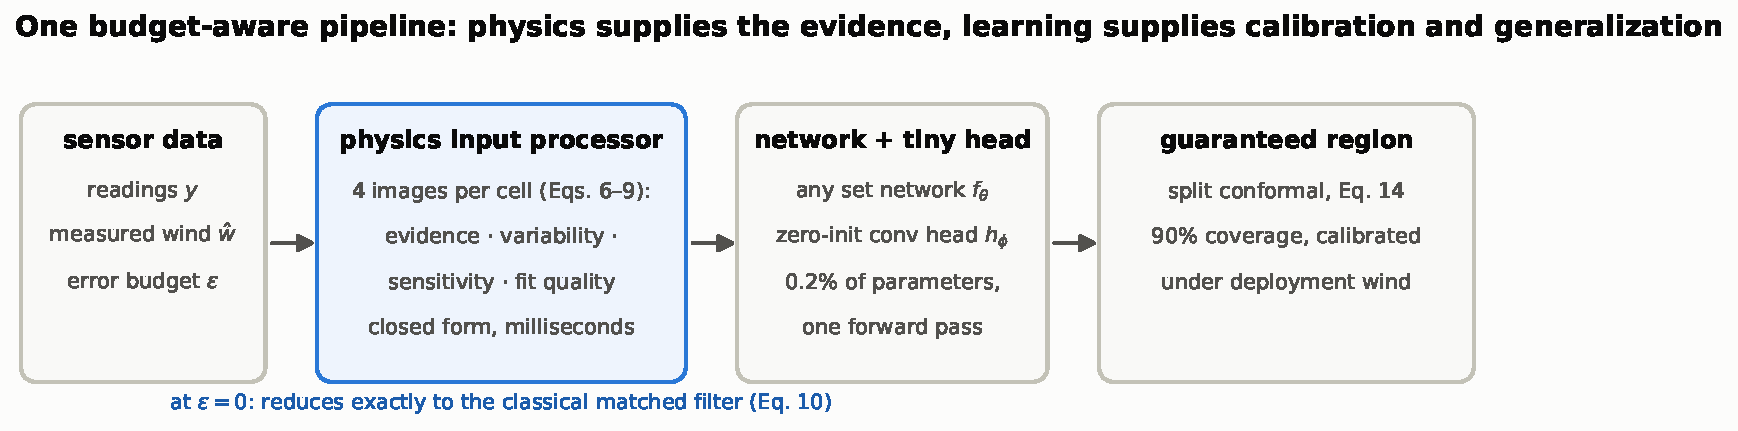
\includegraphics[width=\linewidth]{../figures/poster/poster_pipeline.pdf}

\vspace{10mm}
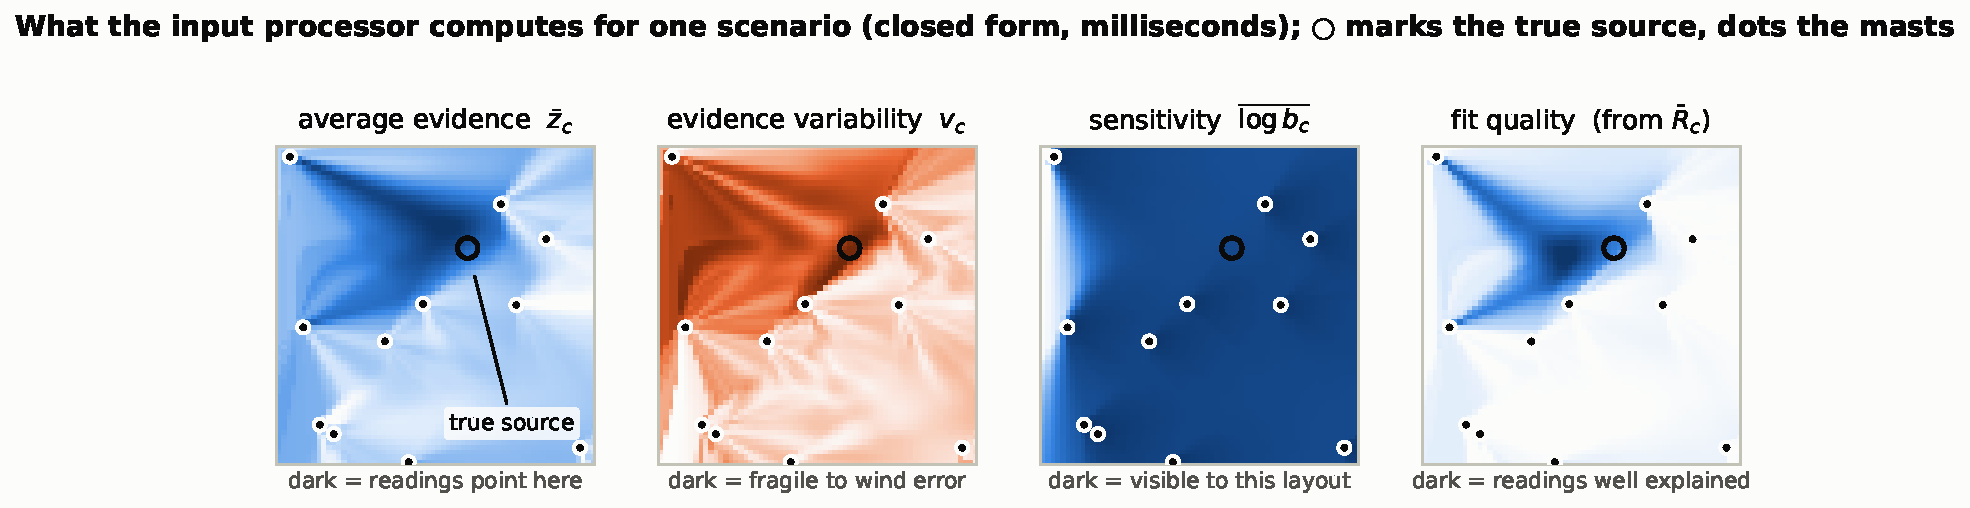
\includegraphics[width=\linewidth]{../figures/poster/poster_maps.pdf}

\vspace{12mm}
\begin{minipage}{0.485\linewidth}\centering
  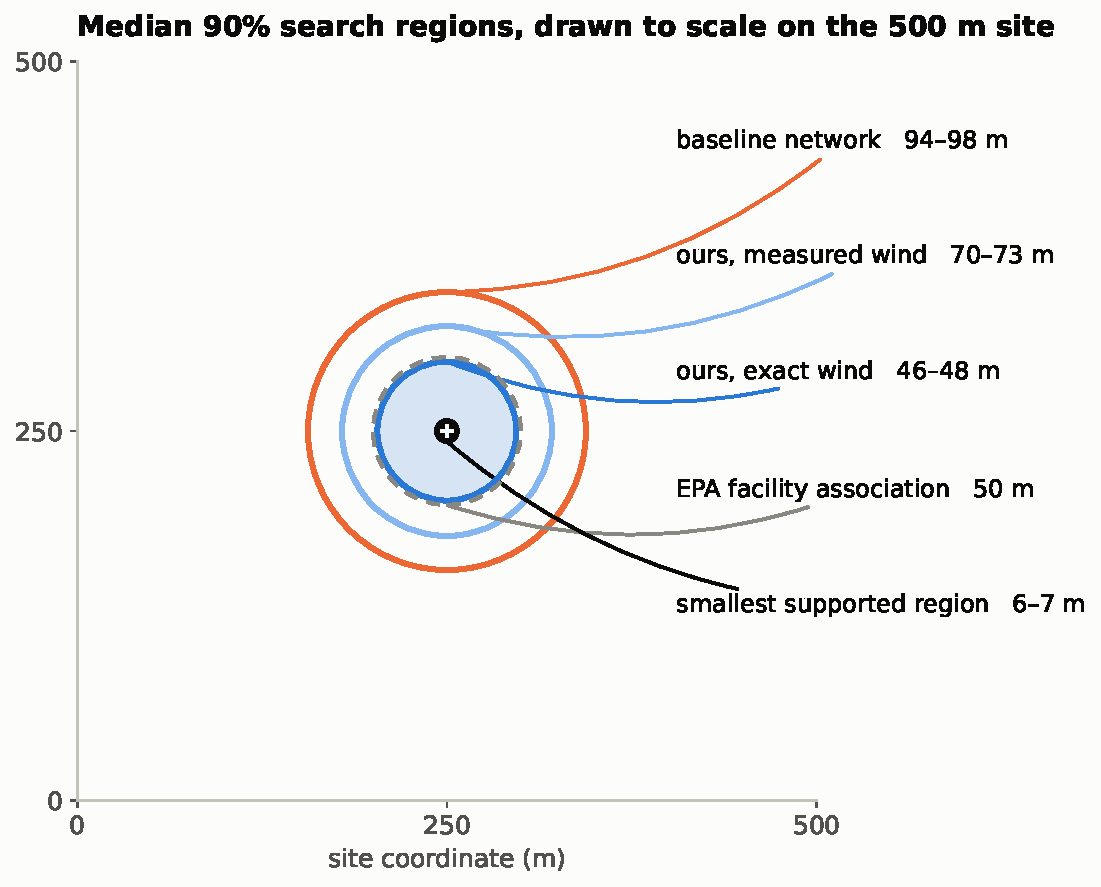
\includegraphics[width=\linewidth]{../figures/poster/poster_scale.pdf}
\end{minipage}\hfill
\begin{minipage}{0.5\linewidth}\centering
  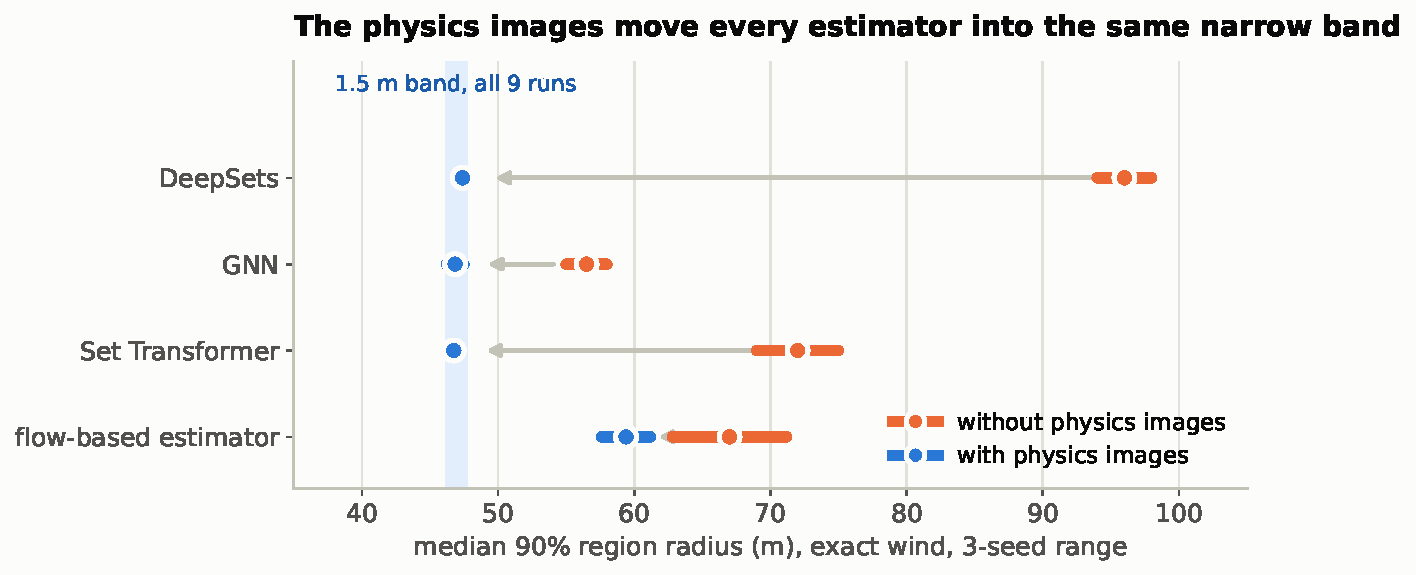
\includegraphics[width=\linewidth]{../figures/poster/poster_dumbbell.pdf}
  \vspace{8mm}
  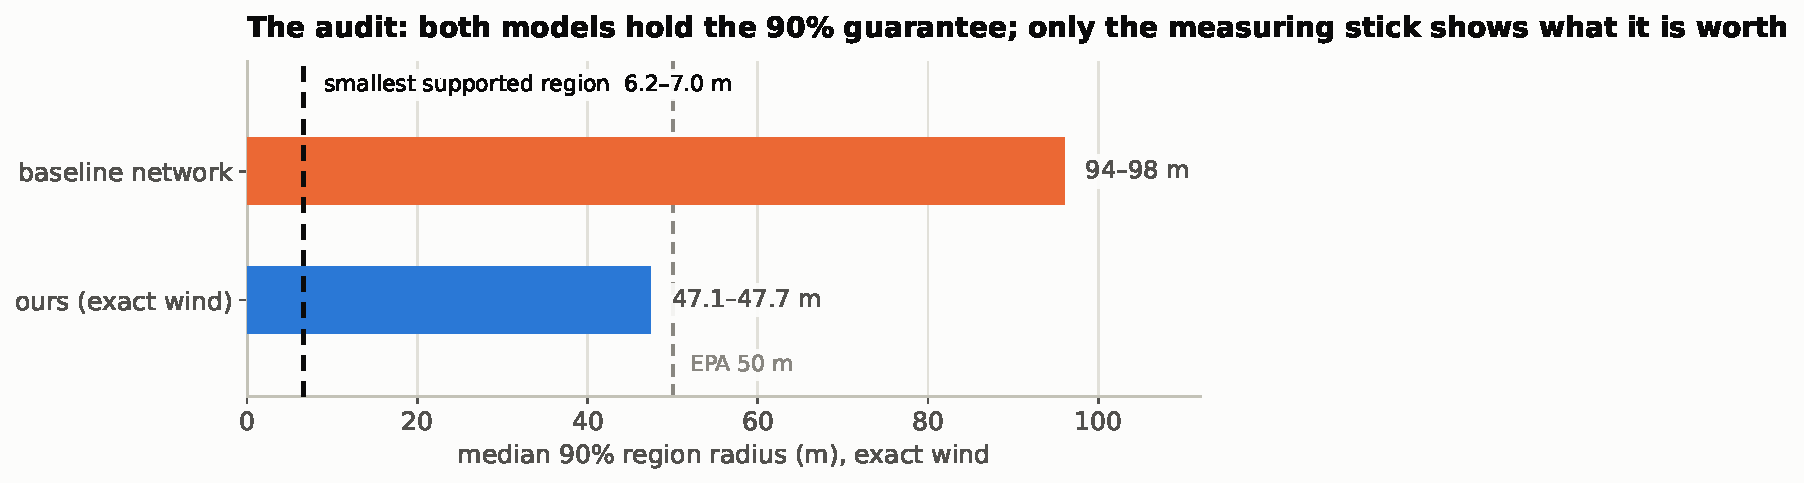
\includegraphics[width=\linewidth]{../figures/poster/poster_audit.pdf}
\end{minipage}

\vspace{12mm}
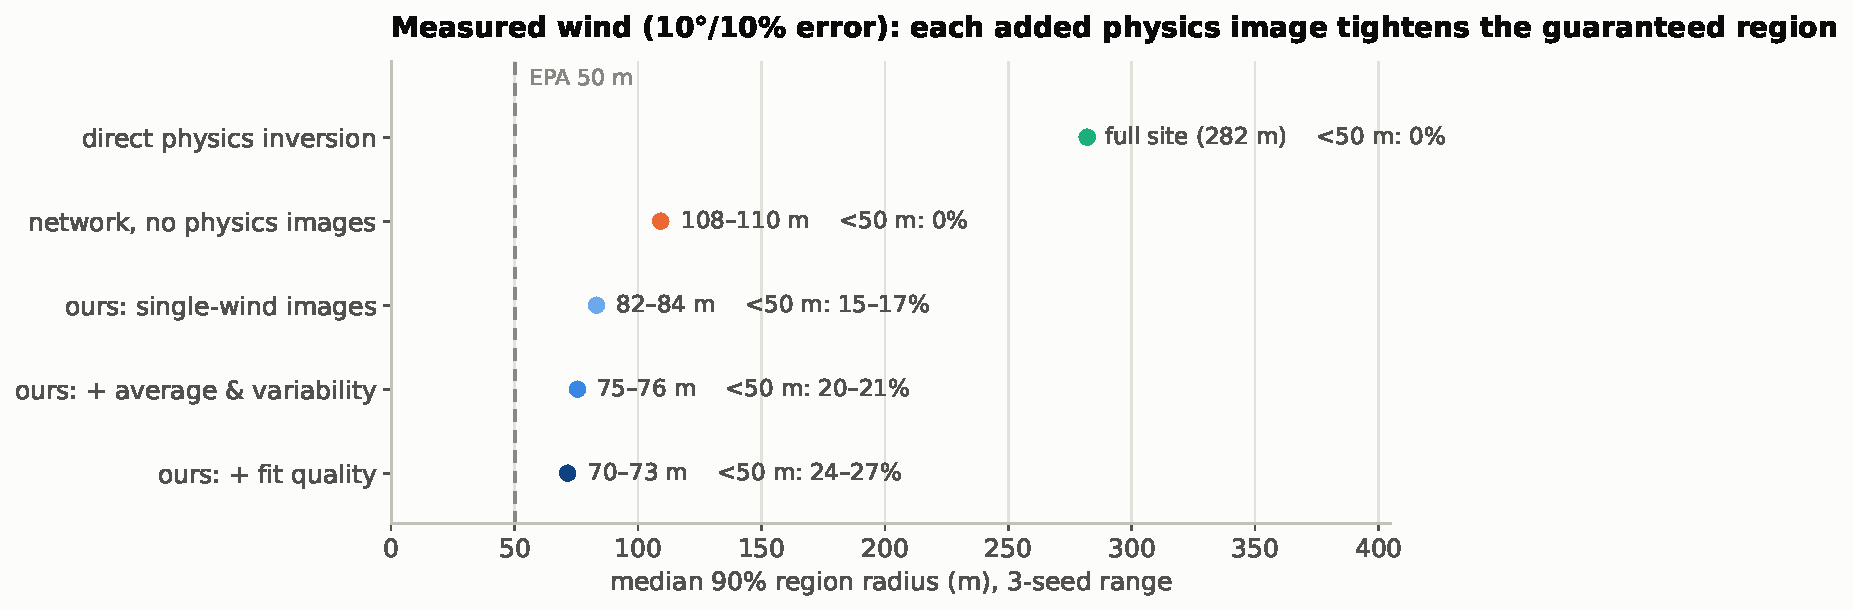
\includegraphics[width=\linewidth]{../figures/poster/poster_ladder.pdf}

\vspace{14mm}
\begin{minipage}{0.57\linewidth}\centering
  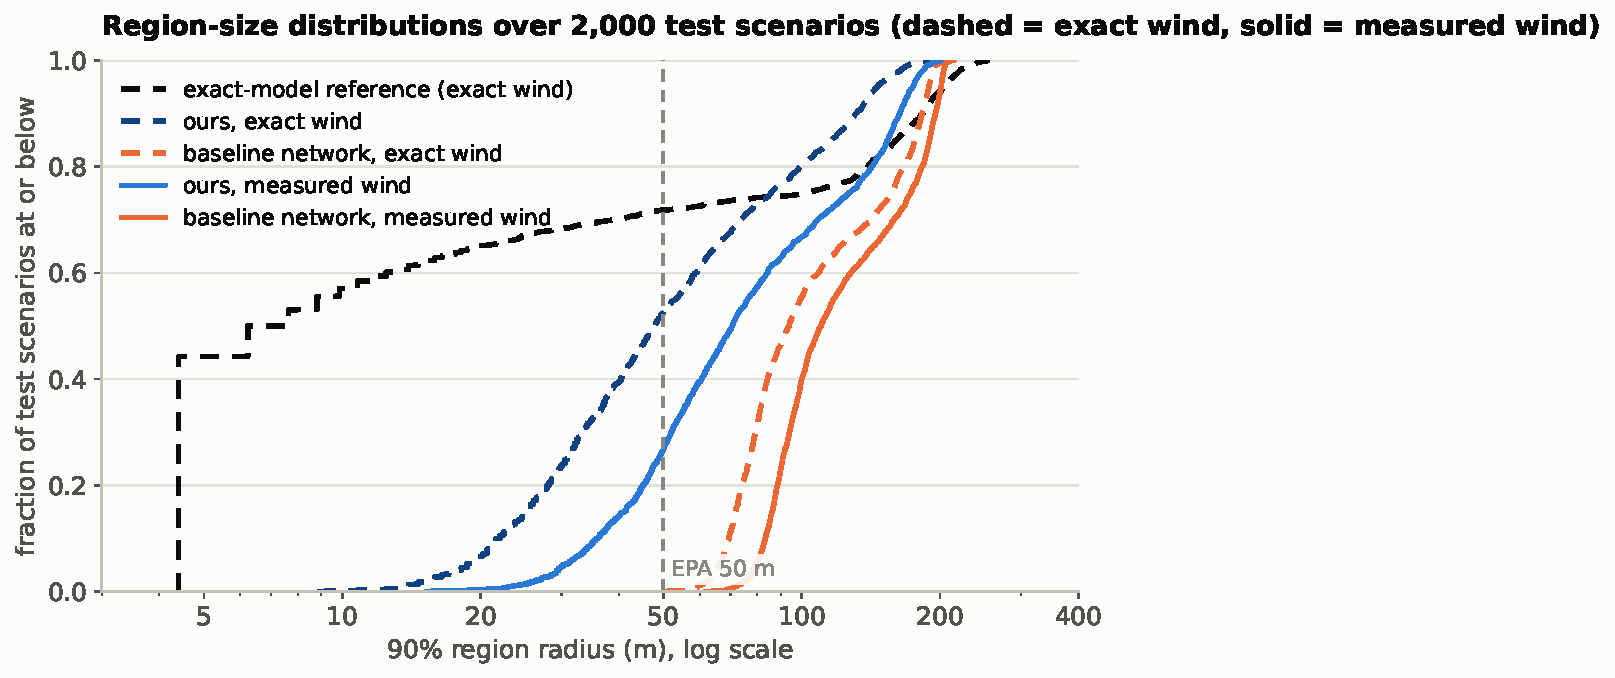
\includegraphics[width=\linewidth]{../figures/paper/fig_data_ecdf.pdf}
\end{minipage}\hfill
\begin{minipage}{0.415\linewidth}\centering
  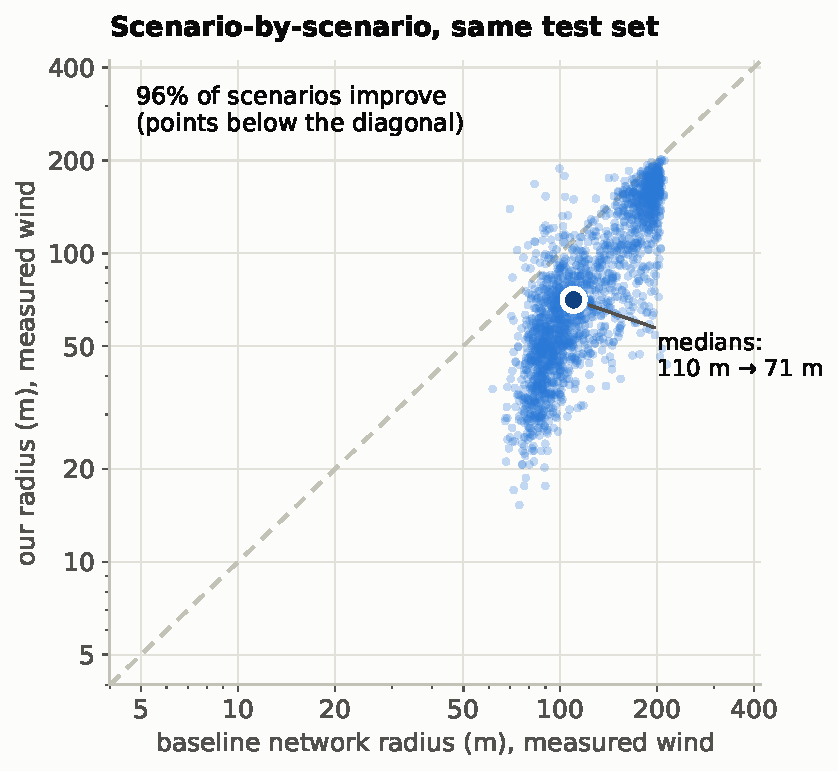
\includegraphics[width=\linewidth]{../figures/paper/fig_data_scatter.pdf}
\end{minipage}

\vspace{14mm}
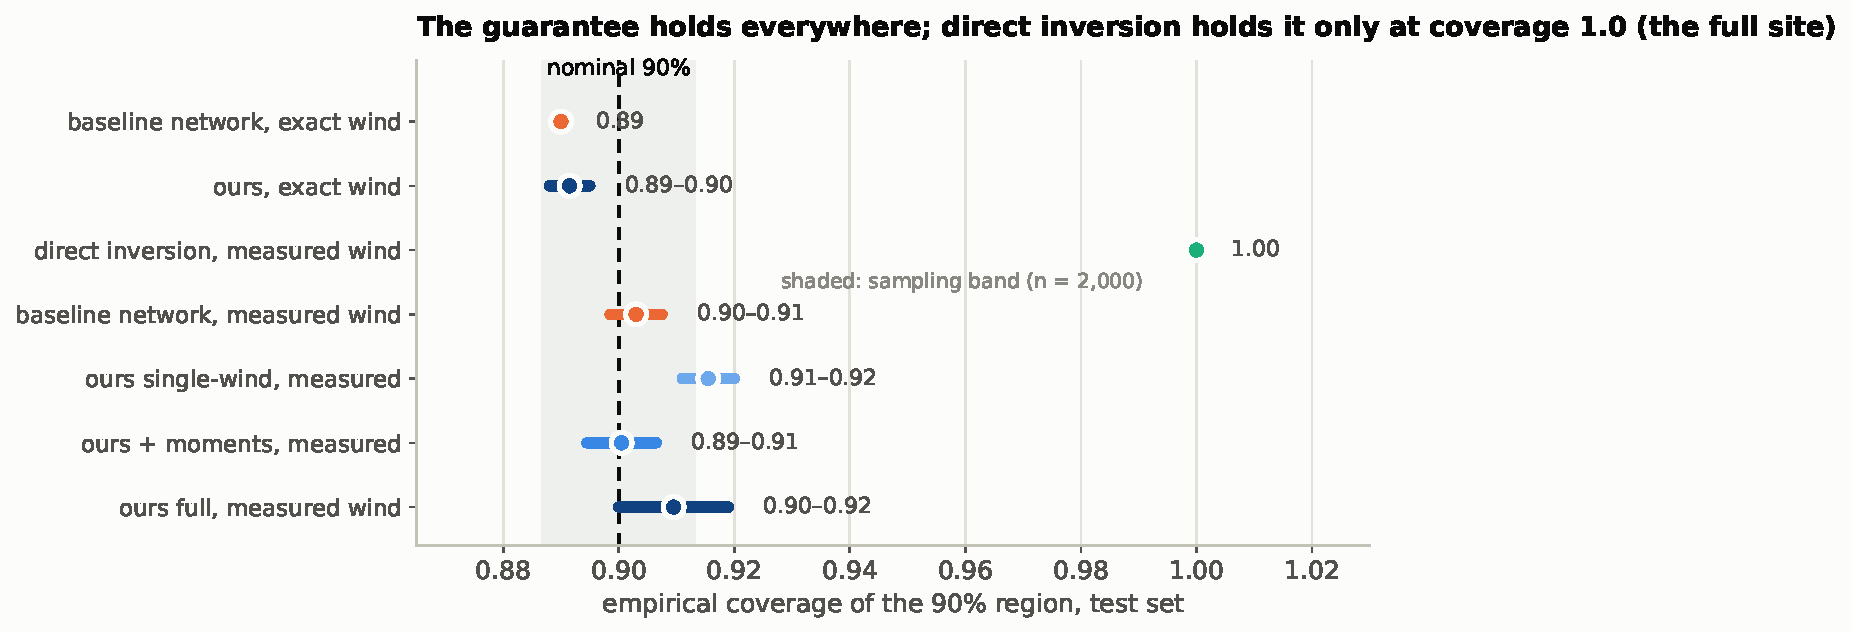
\includegraphics[width=0.98\linewidth]{../figures/paper/fig_data_coverage.pdf}

\vspace{14mm}
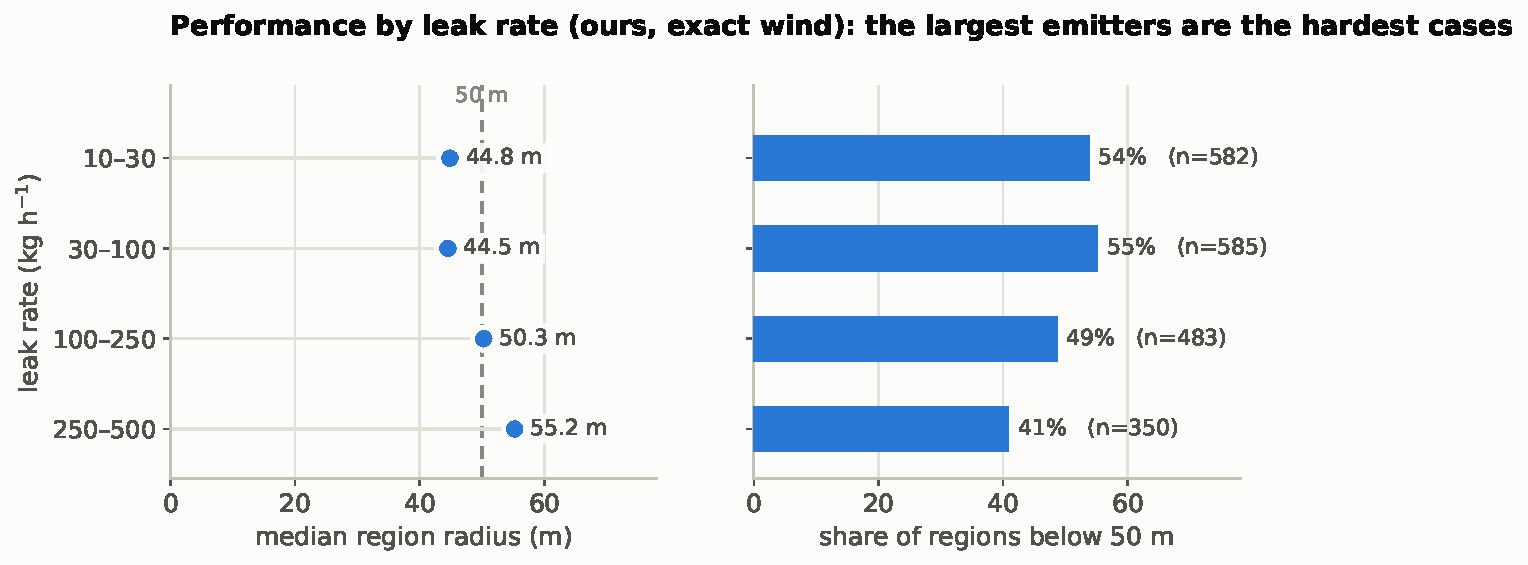
\includegraphics[width=0.9\linewidth]{../figures/paper/fig_data_rates.pdf}
\end{pbox}

\end{column}

% ---------------------------- RIGHT ------------------------------
\begin{column}{0.265\linewidth}

\begin{pbox}{Discussion / Conclusions}
\textbf{Calibrated is not actionable.} Both learned models pass every
calibration check; only the exact-posterior audit shows one delivers
regions $10\times$ larger than the data support.

\srule

\textbf{The fix belongs in the inputs.} Supplying the classical
evidence computation as images moves DeepSets, GNN, and Set Transformer
from a 40\,m spread into a \textbf{1.5\,m band at 46--48\,m}; the same
images improve a flow-based estimator, so the recipe composes with any
architecture.

\srule

\textbf{Wind uncertainty, budgeted honestly.} Under measured wind,
direct inversion keeps its guarantee only by returning the full site.
Each image of wind-error structure tightens the learned regions:
$108 \to 82 \to 75 \to \mathbf{71}$\,m, a quarter of cases below 50\,m,
at one forward pass.

\srule

\textbf{The decomposition.} $94{\to}47$\,m: the missing computation,
fixed by inputs. $47{\to}71$\,m: the price of imperfect wind.
$108{\to}71$\,m: the value of physics when the wind is real.

\srule

\textbf{Limitations \& next steps.} Simulation testbed (single steady
source, flat terrain); error budget assumed known; largest emitters
hardest. Next: misspecified budgets, controlled-release field
validation (METEC-style).
\end{pbox}

\vspace{10mm}

\begin{pbox}{At a Glance}
\centering
\begin{minipage}{0.47\linewidth}\centering
  {\color{navy}\bfseries\Huge 7\,m}\\[1mm]
  {\small what the data support (6--7)}
\end{minipage}\hfill
\begin{minipage}{0.47\linewidth}\centering
  {\color{navy}\bfseries\Huge 47\,m}\\[1mm]
  {\small ours, exact wind (46--48)}
\end{minipage}

\vspace{7mm}
\begin{minipage}{0.47\linewidth}\centering
  {\color{navy}\bfseries\Huge 71\,m}\\[1mm]
  {\small ours, measured wind (70--73)}
\end{minipage}\hfill
\begin{minipage}{0.47\linewidth}\centering
  {\color{navy}\bfseries\Huge 90\,\%}\\[1mm]
  {\small coverage, certified everywhere}
\end{minipage}
\end{pbox}

\vspace{10mm}

\begin{pbox}{References}
\small
[1] U.S.\ EPA, NSPS OOOOb/EG OOOOc \& Super-Emitter Program, 2024.\quad
[2] UNEP IMEO, \emph{An Eye on Methane}, 2024.\quad
[3] Angelopoulos \& Bates, \emph{Conformal Prediction}, FnTML 2023.\quad
[4] Papamakarios \& Murray, NeurIPS 2016.\quad
[5] Cannon et al., \emph{Model Misspecification in SBI}, 2022.\quad
[6] Ilonze et al., \emph{Elementa} 2025 (METEC).
\end{pbox}

\vspace{10mm}

\begin{pbox}{Acknowledgements}
\small We thank the Boston University RISE Practicum program and our
instructors for guidance, and the BU Shared Computing Cluster for
computation. All results are from a shared, verified simulator with
identical data splits and calibration harness, over three training
seeds.
\end{pbox}

\end{column}
\end{columns}

\end{frame}
\end{document}
